\documentclass[12pt]{article}
\usepackage[polish]{babel}
\usepackage[utf8]{inputenc}
\usepackage{tikz}
\usetikzlibrary{trees}
\usepackage{graphicx}
\graphicspath{ {./images/} }
\begin{document}

\begin{flushright}

Laboratoria: piatek, 8:00

Grupa: 13

Informatyka Wydział informatyki i telekomunikacji.

\end{flushright}

\hspace{4cm}

\begin{center}

Algorytmy i Strukrury Danych

Prowadzacy:

Dominik Witczak

\end{center}

\hspace{4cm}

\begin{center}

\textbf{Sprawozdanie do \LARGE}

\hspace{2cm}

\underline{Projektu 4 Algorytmy z powracaniem}

\end{center}

\hspace{30cm}

\begin{flushright}

Autor:

Marcin Wrzaskowski

nr indeksu:

160329

\end{flushright}

\pagebreak

\section{Uzasadnienie wyboru reprezentacji grafu (macierz sasiedztwa): }

    \subsection{Prostota i przejrzystość:}
        Macierz sasiedztwa to dwuwymiarowa tablica, wypełniona 0 $ M[i, j] = 0$ lub 1 $ M[i, j] = 1 $ jeżeli jest 1 to oznacza że wierzchołki i i j sa połaczone krawedzia.

    \subsection{Szybki dostep do krawedzi:}
        Sprawdzenie, czy istnieje krawedź miedzy dwoma wierzchołkami O(1) złożoność czasowa.

    \subsection{Efektywność dla grafów gestych:}
        Macierz sasiedztwa jest efektywna dla grafów gestych.
    \subsection{Łatwość implementacji algorytmów: }
    		Łatwość implementacji algorytmów dla znajdywania cyklu Eulera/Hamiltona w grafie.
        
\section{Wizualizacje grafów: }

\subsection{Graf hamiltonowski o $|V| = 10$}

\begin{center}

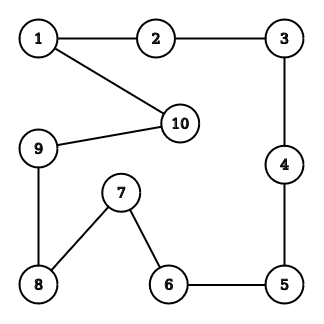
\includegraphics[scale=0.5]{graph_hamilton.png}

\end{center}

\subsection{Graf nie hamiltonowski o $|V| = 10$}

\begin{center}

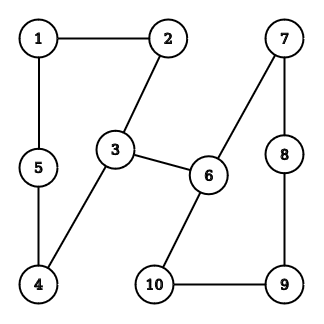
\includegraphics[scale=0.5]{graph_non_hamilton.png}

\end{center}

\section{Wykresy zależności: (dla grafów hamiltonowskich o nasyceniu 30) $ t = f(n) $}

\subsection{Skala liniowa t(ms): }

\begin{center}

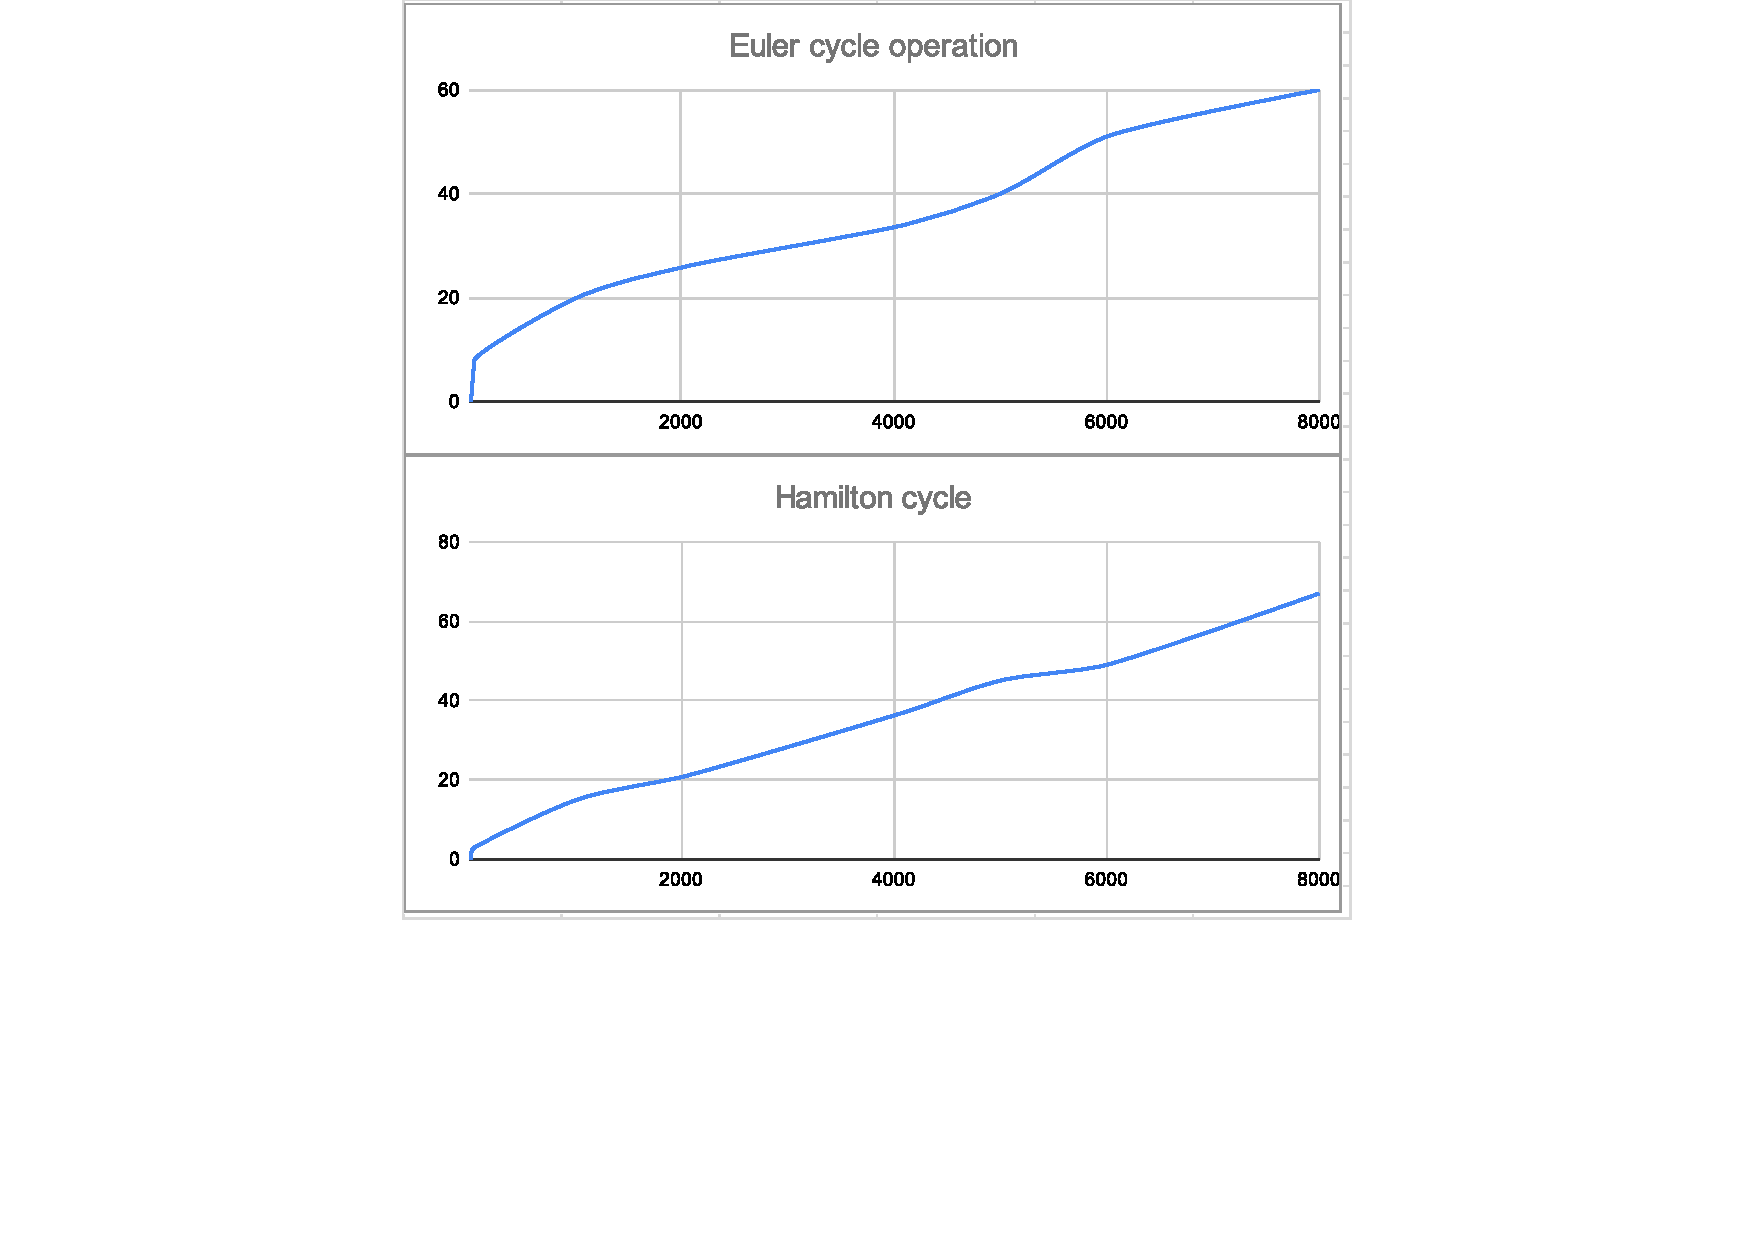
\includegraphics[scale=0.5]{wykres_liniowy_0.pdf}

\end{center}

\subsection{Skala logarytmiczna t(ms): }

\begin{center}

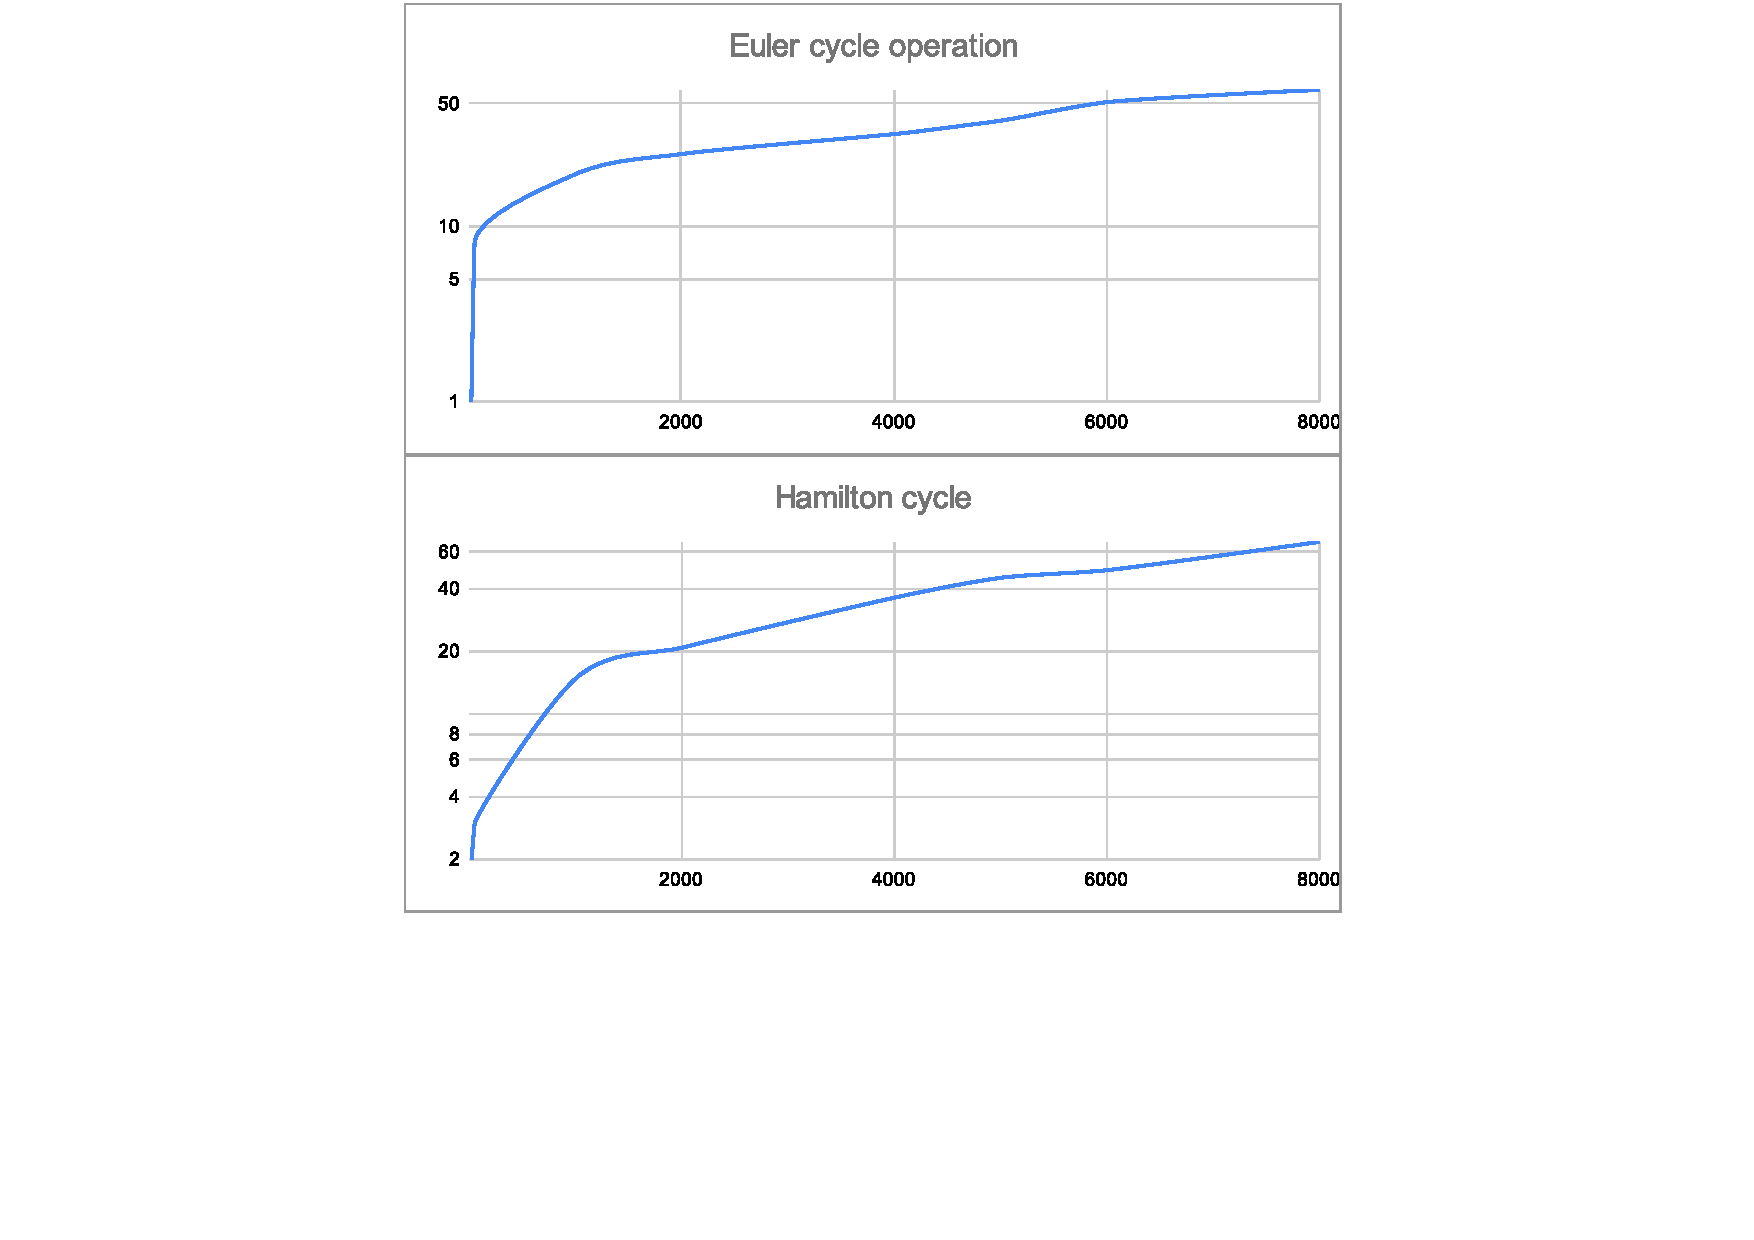
\includegraphics[scale=0.5]{wykres_logarytmiczny_0.pdf}

\end{center}

\section{Wykresy zależności: (dla grafów nie hamiltonowskich o nasyceniu 50) $ t = f(n) $}

\subsection{Skala liniowa t(ms): }

\begin{center}

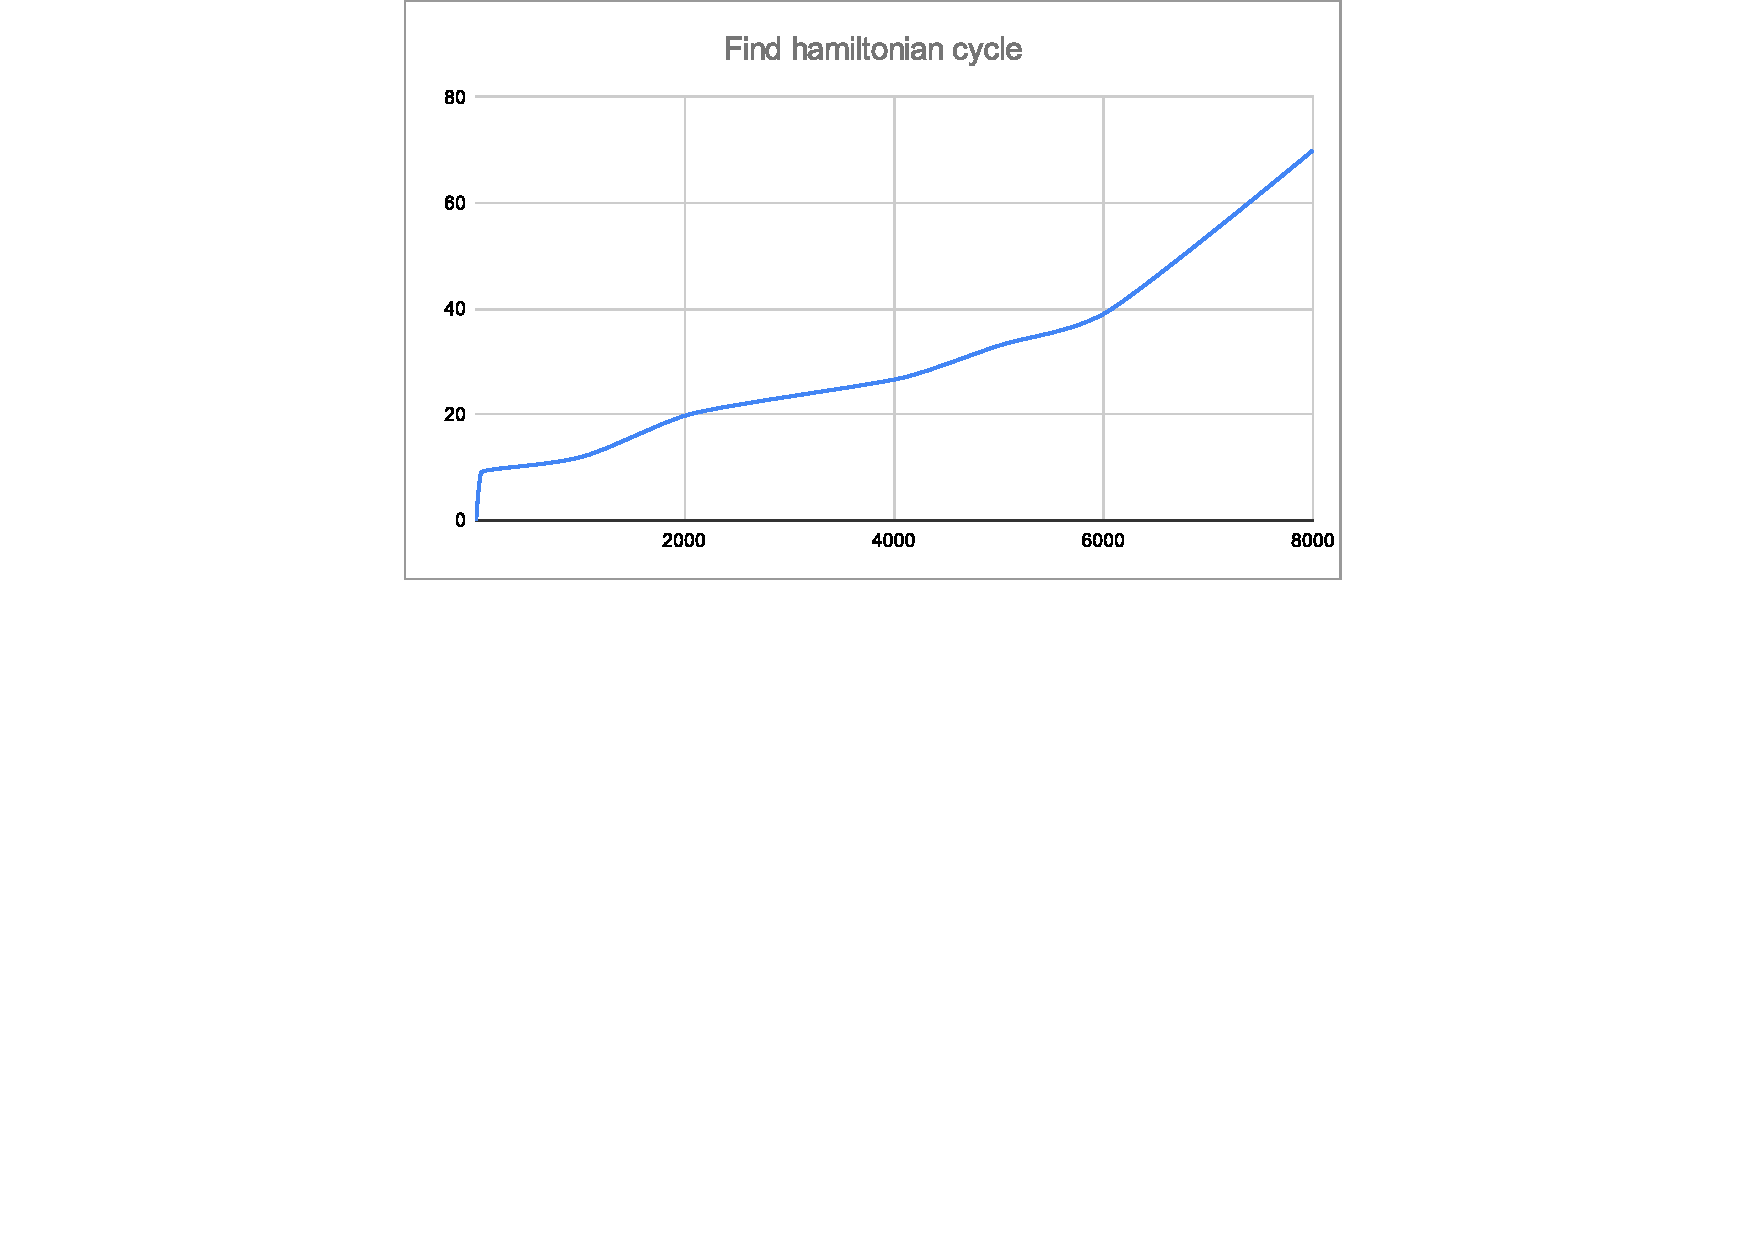
\includegraphics[scale=0.5]{wykres_liniowy_1.pdf}

\end{center}

\subsection{Skala logarytmiczna t(ms): }

\begin{center}

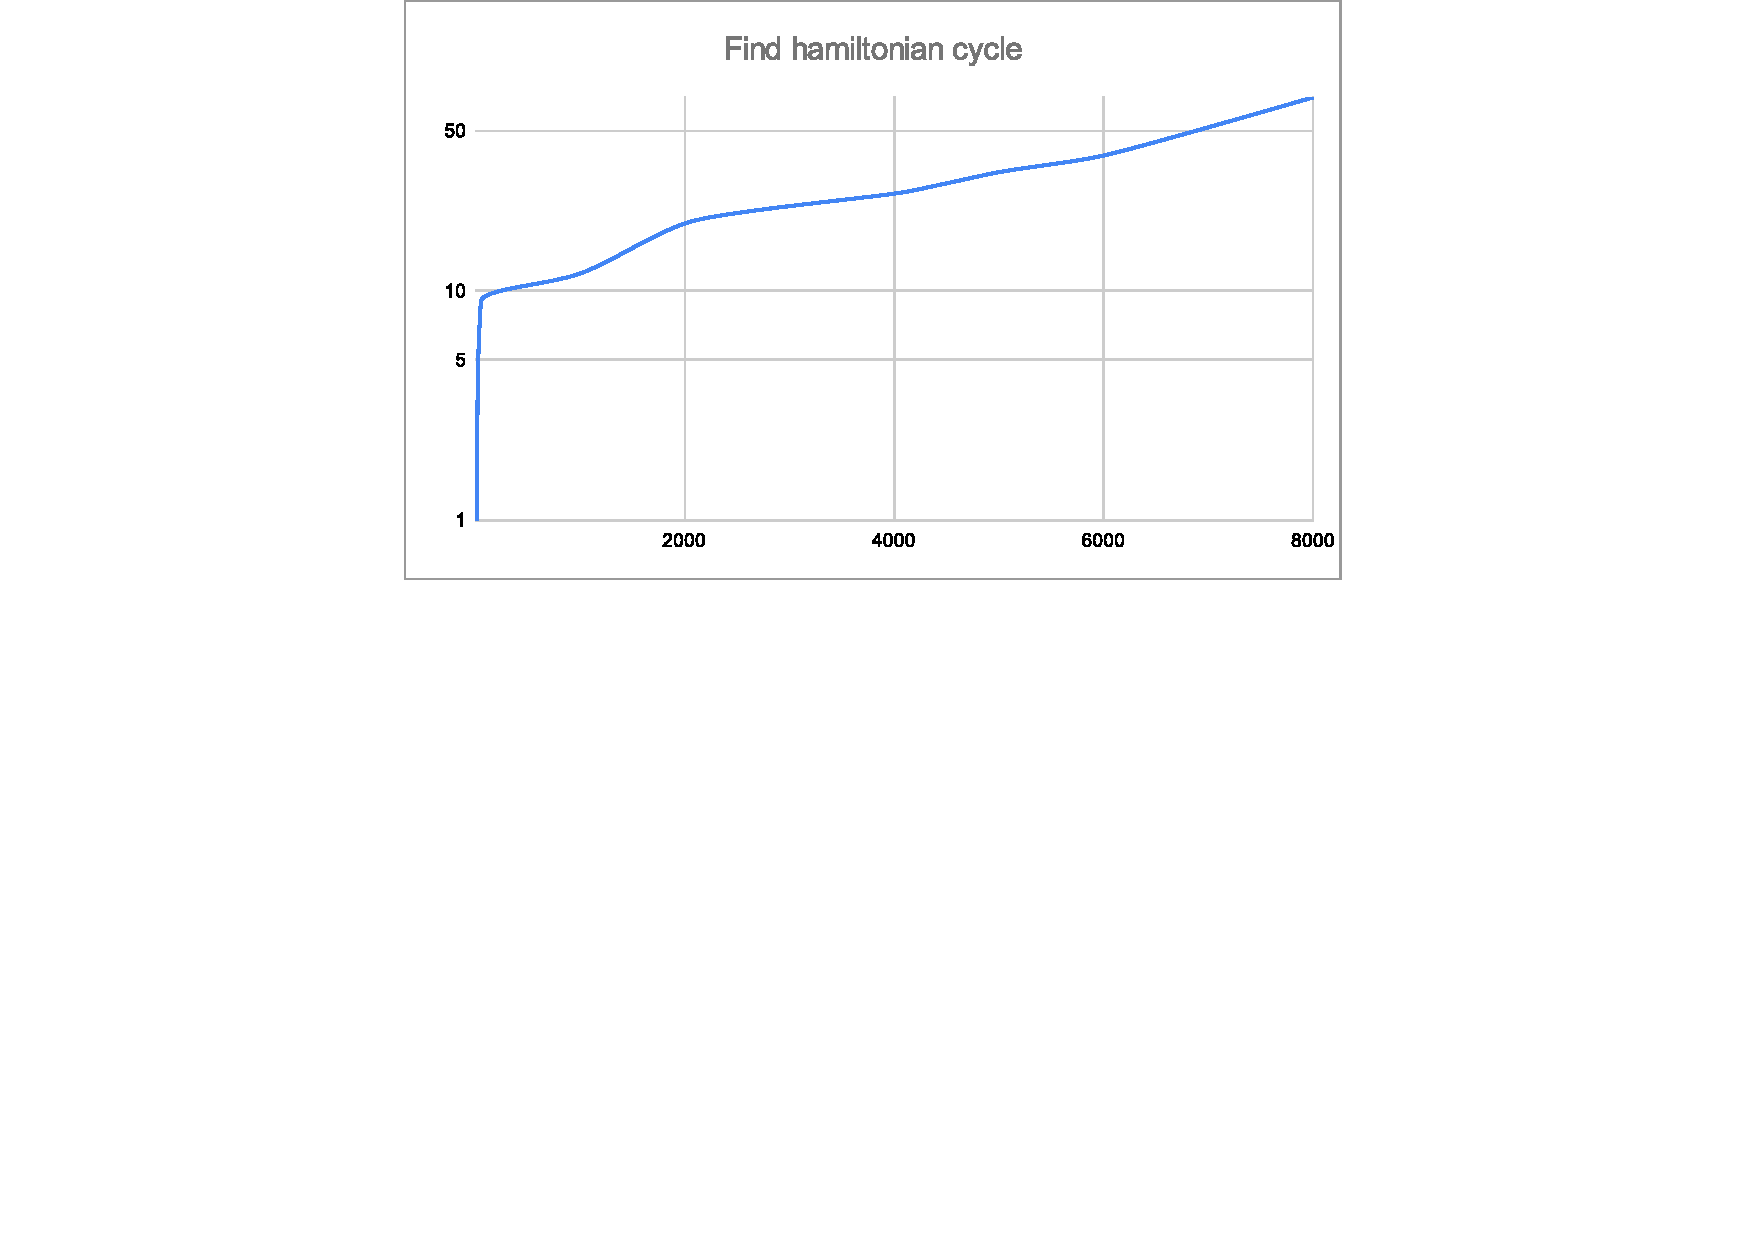
\includegraphics[scale=0.5]{wykres_logarytmiczy_1.pdf}

\end{center}

\section{Obserwacje zwiazane z działaniem obu algorytmów w zależności od nasycenia grafu: }

\begin{enumerate}

	\item 
			Dla grafów o nasyceniu $30\%$, wraz ze wzrostem ilości wierzchołki w grafie czas t rośnie wolniej niż dla grafów o nasyceniu $50\%$.
	\item
			Wnioskujac z poprzedniego punktu te algorytmy (znajdowanie: cyklu Eulera, Hamiltona) dla grafów grafów o nasyceniu $30\%$ działaja szybciej niż dla grafów grafów o nasyceniu $50\%$

\end{enumerate}


\section{Podsumowanie: }

Nauczyłem sie

\begin{enumerate}

	\item
	      Generować grafy hamiltonowskie i nie hamiltonowskie.
	\item
		  Implementowac algorytmy ktore znajduja cykl Eulera, Hamiltona w grafach.
	\item
		  O grafach jako strukturach danych.
    \item
    	      Wypisywania na ekran.
  	\item
  		  Wybierać odpowiednia implementacje maszynowa w zależności od rodzaju problemu do rozwiazania.

\end{enumerate}

\tableofcontents

\end{document}